\documentclass[12pt]{beamer}

\usetheme{CambridgeUS}
\usepackage[utf8]{inputenc}
\usepackage{lmodern}

\begin{document}

\frame {
    \maketitle
}

% Begin Joan Vilà

\frame {
    \frametitle{Instalación: tiempo y problemas}
    \begin{itemize}
        \item {Windows 10}
        \item {Ubuntu}
        \item {Mac OS}
    \end{itemize}
}

\frame {
    \frametitle{Instalación de Windows}
    \begin{enumerate}
        \item {Descargar la ISO (v10 3,71GB)}
        \item {Grabar en un CD o USB}
        \item {Reiniciar arrancando desde CD o USB}
        \item {Instalar medinte boton de siguiente}
        \item {Conseguir o tener una licencia válida y demostrarlo}
    \end{enumerate}
}

\frame {
    \frametitle{Instalación de Ubuntu}
    \begin{enumerate}
        \item {Descargar la ISO (v16.04 1,51GB)}
        \item {Grabar en un CD o USB}
        \item {Reiniciar arrancando desde CD o USB}
        \item {Instalar medinte boton de siguiente}
    \end{enumerate}
}

\frame {
    \frametitle{Instalación de MacOS}
    \begin{enumerate}
        \item {Reiniciar en modo recuperación}
        \item {Seleccionar reinstalar el SO}
        \item {Esperar (vSierra 4,86GB)}
    \end{enumerate}
}

\frame {
    \frametitle{Ventajas de cada uno}
    \begin{itemize}
        \item {Windows: ???}
        \item {Ubuntu: Gratis, posibilidad de instalarlo al lado de otros SO}
        \item {MacOS: Facil, nivel usuaro bajo}
    \end{itemize}
}

\frame {
    \frametitle{Desventajas de cada uno}
    \begin{itemize}
        \item {Windows: Grabar la ISO y el precio/licencia}
        \item {Ubuntu: Grabar la ISO}
        \item {MacOS: Tiempo de descarga}
    \end{itemize}
}

\frame {
    \frametitle{Aplicaciones disponibles y coste}
    \textbf{Comparación entre Windows Store, ubuntu sofware center y mac AppStore}
}

\frame {
    \frametitle{Windows Store}
    \begin{itemize}
        \item {669.000 apps para moviles, ordenadores y tabletas}
        \item {Ojo! Sólo aplicaciones universales}
    \end{itemize}
}

\frame {
    \frametitle{Ubuntu Software Center}
    \begin{itemize}
        \item {Número de apps desconocido}
        \item {El número depende de las fuentes en las que se confie}
        \item {Posibilidad de añadir y quitar fuentes a gusto}
    \end{itemize}
}

\frame {
    \frametitle{Mac App Store}
    \begin{itemize}
        \item {31.191 apps disponibles para Mac}
        \item {Estricto filtro para colgar una app}
        \item {Travas para utilizar apps de terceros}
    \end{itemize}
}

\frame {
    \frametitle{Comparando las alternativas}
    \begin{itemize}
        \item {Windows: necesidad de buscar la vida por internet}
        \item {Mac: utilizar Homebrew como fuente de software y buscar la vida por internet}
        \item {Ubuntu: Difícil compatibilidad con software privativo de las otras plataformas}
    \end{itemize}
}

\frame {
    \frametitle{Comparativa de precios}
    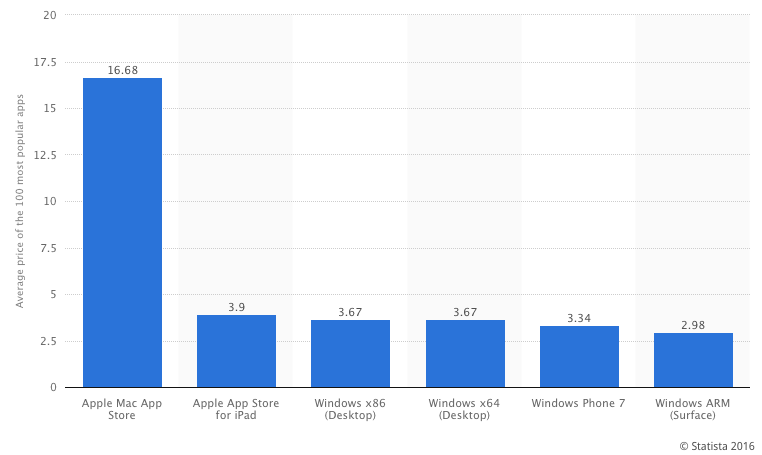
\includegraphics[width=\textwidth]{PriceComparison.png}
}

\frame {
    \frametitle{Reflexión de problemas vistos hasta el momento}
    \begin{itemize}
        \item {Windows: Software propenso a virus y con problemas de privacidad}
        \item {Mac: Hacks como Homebrew para acceder a fuentes de software y problemas de privacidad}
        \item {Ubuntu: No es posible utilizar sofware popular de Microsoft, Adobe... (wine)}
    \end{itemize}
}

% End Joan Vilà
% Begin Sergi Soriano

\frame {
    \frametitle{Velocidad de arranque / ejecución de aplicaciones / copias}
    \textbf{Sergi Soriano}
}

% End Sergi Soriano
% Begin Miquel Xamani

\frame {
    \frametitle{Uso de recursos del sistema (usuario y/o servidor)}
    \textbf{Miquel Xamani}
}

% End Miquel Xamani
% Begin Arnau Garcia

\frame {
    \frametitle{Comparativa de tiempos/recursos para una aplicación en el mismo PC bajo distintos SO}
    \framesubtitle{Introducción}
    \begin{itemize}
    \item {Interacción entre los componentes del sistema operativo y el tiempo de ejecución sigue siendo en parte un misterio}
    \end{itemize}
    \begin{enumerate}
    \item{Fallos de la memoria de traducción (TLB)}
    \item{Interrupciones}
    \item{Eventos asíncronos}
    \end{enumerate}
    \begin{itemize}
    \item{Pueden \textbf{afectar al rendimiento} de los SO}
    \end{itemize}
}
\frame {
    \frametitle{Comparativa de tiempos/recursos para una aplicación en el mismo PC bajo distintos SO}
    \framesubtitle{Introducción}
    \begin{itemize}
    \item {\textbf{Ruido}: interferencia del sistema operativo}
    \item{Importante intentar definir/interpretar lo que consideramos ruido:}
    \end{itemize}
    \large{\emph{"Colección de actividades de fondo que involuntariamente interrumpen el progreso de la aplicación principal.”}}
}


% End Arnau Garcia
% Begin Guillem Gordillo

\frame {
    \frametitle{Posibilidades de simulación / virtualización en unos y otros. Interoperabilidad}
    \textbf{Guillem Gordillo}
}

% End Guillem Gordillo

\frame {
    \frametitle{Bibliografía}
    \begin{itemize}
        \item {http://informatica.blogs.uoc.edu/2016/03/08/guia-para-elegir-el-sistema-operativo-de-tu-ordenador-windows-os-x-o-linux/}
        \item {http://www.howtogeek.com/197559/how-to-install-windows-10-on-your-pc/}
        \item {https://help.ubuntu.com/community/Installation}
        \item {https://support.apple.com/en-us/HT204904}
        \item {http://venturebeat.com/2016/03/30/hey-microsoft-how-many-apps-are-in-the-windows-store/}
        \item {https://wiki.ubuntu.com/SoftwareCenter}
    \end{itemize}
}

\end{document}
